\documentclass[12pt]{article}
\usepackage{mathptmx}
\usepackage{fullpage}
\usepackage{multicol}
\usepackage{amsmath,amssymb}
\usepackage{graphicx}
\usepackage[aux]{rerunfilecheck}

\newcommand{\ds}{\displaystyle}

\reversemarginpar

\title{MATH 110-004 200730 Quiz 5 Solutions}
\author{Edward Doolittle}

\begin{document}
\maketitle

\begin{enumerate}
\item In Figure~\ref{fig:ships}, ship $A$ moves `west' along the $x$-axis
  and ship $B$ moves `north' along the $y$ axis.
  \begin{figure}
    $\begin{array}{c@{\hspace{0.25in}}c}
      \includegraphics{ships0.eps} & \includegraphics{ships1.eps} \\
      \mbox{time $t= $ noon}       & \mbox{time $t= $ 4:00 pm}
    \end{array}$
    \caption{Position of ships at noon and 4:00 pm}
    \label{fig:ships}
  \end{figure}
  We have the Pythagorean relation among the variables $x$, $y$, and $z$:
  \begin{align*}
    x^2+y^2=z^2
  \end{align*}
  Differentiating with respect to time,
  \begin{align*}
    2x \frac{dx}{dt} + 2y \frac{dy}{dt} = 2z\frac{dz}{dt}
  \end{align*}
  From the given data, at 4:00 pm we have $dx/dt=-10$, $x=-35-4(10)=-75$, 
  $dy/dt=25$, $y=0+4(25)=100$.
  We can calculate $z$ using the Pythagorean relation:
  $z^2=x^2+y^2=75^2+100^2=125^2$.  Since the distance must be positive we
  have $z=125$.  Filling in that data we have
  \begin{align*}
    -75\cdot -10 + 100\cdot 25 = 125 \cdot \frac{dz}{dt}
    \implies \frac{dz}{dt} = 26
  \end{align*}
  The ships are moving away from each other at a rate of $26$ km/h at 4:00 pm.
\item 
  \textbf{Solution 1:} The relations among the dimensions
  of the sphere are
  \begin{align*}
    C = 2\pi r    \qquad A = 4\pi r^2      \qquad  V = \frac{4}{3} \pi r^3
  \end{align*}
  Differentiating,
  \begin{align*}
    dC = 2\pi dr  \qquad dA = 8\pi r \; dr \qquad dV = 4\pi r^2 \; dr
  \end{align*}
  We are given $C=84$ and $dC=0.5$.  Solving for $r$ and $dr$ using the
  first set of relations,
  $r=84/2\pi \approx 13.4$, $dr=0.5/2\pi \approx 0.080$, so
  \begin{align*}
    dA = 8\pi r \; dr \approx 26.9 \qquad dV = 4\pi r^2 \; dr \approx 180
  \end{align*}
  So the maximum error in the calculated value of the surface area is about
  $26.9$ cm$^2$ and the maximum error in the calculated value of the volume
  is about $180$ cm$^3$.

  Since $A=4\pi r^2 \approx 2260$ cm$^2$, the relative error in the value of
  $A$ is about $dA/A=0.012$ or about 1.2\%.  Since $V=(4/3)\pi r^3\approx
  10100$ cm$^3$, the relative error in $V$ is about $dV/V\approx 180/10100
  \approx 0.018$ or about 1.8\%.

  \textbf{Solution 2:} We can find formulas for $A$ and $V$ in terms of $C$
  without $r$.  We have $r=C/2\pi$ so 
  \begin{align*}
    A = 4\pi r^2 = 4\pi \left(\frac{C}{2\pi}\right)
    = 4\pi \frac{C^2}{4\pi^2} = \frac{C^2}{\pi}
    \qquad
    V = \frac{4}{3} \pi r^3
    = \frac{4}{3} \pi \left(\frac{C}{2\pi}\right)^3
    = \frac{4}{3} \pi \frac{C^3}{8\pi^3}
    = \frac{C^3}{6\pi^2}
  \end{align*}
  Differentiating,
  \begin{align*}
    dA = \frac{2}{\pi} C \; dC
    \qquad
    dV = \frac{1}{2\pi^2} C^2 \; dC
  \end{align*}
  Substituting $C=84$ and $dC=0.5$ we have
  \begin{align*}
    dA = \frac{2}{\pi} 84\times 0.5 \approx 26.7
    \qquad
    dV = \frac{1}{2\pi^2} (84)^2 \times 0.5 \approx 179.
  \end{align*}
  So the errors in the calculated values of the surface area and volume are
  about $26.7$ cm$^2$ and $179$ cm$^3$ respectively.

  Since $A=C^2/\pi\approx 2250$ cm$^2$, 
  the relative error in $A$ is approximately
  $dA/A\approx 26.7/2250\approx 0.012$ or 1.2\%.
  Since $V=C^3/6\pi^2\approx 10000$ cm$^3$, the relative error in $V$
  is approximately $dV/V\approx 0.018$ or about 1.8\%.
\end{enumerate}

\end{document}


